\chapter{Lepton Flavour in the Standard Model and Beyond}\label{chapter1}

% Crazy superlatives about the SM
The Standard Model (SM) of particle physics is possibly the most successful
mathematical model of physical phenomena so far. It provides an accurate
description of almost all observable interactions between known elementary
particles. It yields predictions for what nature does and does not allow, and
enables physicists to examine and test the fundamental laws of the universe.
Furthermore, the SM establishes a rigid framework to make theoretical
predictions, from which any measured deviations can then be interpreted as new
physics.

The conservation of lepton flavour, which stems from an accidental symmetry of the SM,
is currently under strict scrutiny by various experiments around the world. 
The observation of neutrino oscillations has already proven that lepton flavour
is not conserved by neutral leptons, and this has driven the search for lepton
flavour violation among the charged leptons. If it is observed, not only will it
add to the current evidence that the SM is incomplete, but it will help guide us
toward the next theory of particle physics beyond the Standard Model.

The most sensitive probe to search for charged lepton flavour violation (CLFV)
is the muon, in large part because muons can be readily produced and focused
into intense beams at accelerator facilities. This chapter describes how the
muon has come from being a mysterious particle showering Earth from outer space
to becoming a tool in high energy physics experiments used to explore the
frontier of our knowledge of nature.


\section{Discovery of the muon}
The first traces of muons were observed around 1937 by three experiments
investigating the nature of cosmic ray-induced particle
showers~\cite{PhysRev.51.884, PhysRev.52.1198, PhysRev.52.1003}. One of them was
able to estimate the mass of the discovered particle at hundreds of times that of the
electron: around the same as the strong-force-carrying meson predicted by Yukawa
in 1935~\cite{10.1143/PTPS.1.1}. Hence, the muon and Yukawa's particle were
originally believed to be one and the same particle. It was only a decade later,
when the meson (now called $\pi$, for primary) was observed decaying into a
muon, that the two particles were completely disambiguated~\cite{LATTES1947}.

It was the fact that the muon appeared as nothing but a heavy electron which
prompted Rabi to ask ``who ordered that?'' in response to its discovery. In
fact, even the Standard Model of today cannot give a satisfactory answer to this
question, since the SM does not motivate the existence of three generations of
elementary particles. As far as the SM can explain, there is no fundamental reason
for the existence of distinct flavours.

\section{The muon in the Standard Model}
% 
The SM identifies the muon as the second-generation charged lepton, meaning it
is a fermion with identical properties, aside from flavour and mass, as the electron
and tau lepton. A muon in a vacuum can only decay through the weak force. The
diagram for muon decay, $\mu^- \rightarrow e^- +  \nu_\mu + \overline{\nu}_e$,
is shown in Fig.~\ref{fig:weak_decay}.


\begin{figure}
    \centering
    \feynmandiagram [layered layout, horizontal=a to b] {
        a [particle=\(\mu^{-}\)] -- [fermion] b -- [fermion] f1 [particle=\(\nu_{\mu}\)],
        b -- [boson, edge label'=\(W^{-}\)] c,
        c -- [anti fermion] f2 [particle=\(\overline \nu_{e}\)],
        c -- [fermion] f3 [particle=\(e^{-}\)],
    };
    \caption{Feynman diagram for the weak decay of the muon.}
    \label{fig:weak_decay}
\end{figure}

In the SM Lagrangian with massless neutrinos, none of the terms which involve
leptons allow for flavour violation. The Lagrangian is invariant under
transformations of the ${U(1)_e \times U(1)_\mu \times U(1)_\tau}$ group.
Consequently, each lepton family ($e$, $\mu$, $\tau$) has its own conserved
number. In theory, this completely prevents a charged lepton from changing
flavour without neutrinos being involved to balance the process. 

These conservation laws do not correspond to a fundamental symmetry of nature;
they are merely an accidental feature of the SM Lagrangian and have, so far,
been observed to hold experimentally. For instance, the process ${\mu
\rightarrow e + \gamma}$, in principle allowed by kinematics, has never been
observed and the current upper limit on its branching ratio was set by the MEG
experiment at $10^{-13}$~\cite{mori2016final}.

The observation of neutrino oscillations~\cite{PhysRevLett.81.1562} means that
the three accidental flavour symmetries are not exact. This strongly motivates a
search for flavour violation among the charged leptons as well, as any evidence
for it would yield additional hints about the theory lying beyond the Standard
Model (BSM).

\begin{figure}
\centering
\begin{subfigure}[t]{0.45\textwidth}
    \centering
    \begin{tikzpicture}
    \begin{feynman}
    \vertex (a) {\(\mu\)};
    \vertex [right=1.5cm of a] (b);
    \vertex [right=1.8cm of b] (c);
    \vertex [right=1.5cm of c] (d) {\(e\)};
    
    \vertex at ($(b)!0.5!(c) + (0, 0.9cm)$) (n);
    \vertex at ($(b)!0.5!(c) + (0, -0.9cm)$) (w);
    \vertex [above=0.1cm of w] (wn) {\(W\)};
    \vertex [below=1.5cm of d] (g) {\(\gamma\)};
    
    \diagram* {
    (a) -- [fermion] (b)
    -- [fermion, quarter left, edge label=\(\nu_\mu\)] (n)
    -- [fermion, quarter left, edge label=\(\nu_e\)] (c),
    (b) -- [boson, quarter right] (w)
    -- [boson, quarter right] (c),
    (c) -- [fermion] (d),
    (w) -- [boson] (g),
    };
    
    \draw (n) -- (n) node {\(\times\)};
    
    \end{feynman}
    \end{tikzpicture}
    \caption{
        $\mu \rightarrow e + \gamma$
    }
    \label{fig:mu_e_nu_osc}
\end{subfigure}
\begin{subfigure}[t]{0.45\textwidth}
    \centering
    \begin{tikzpicture}
    \begin{feynman}
    \vertex (m1) {\(\mu\)};
    \vertex [right =1.5cm of m1] (m2);
    \vertex [right =1.8cm of m2] (m3);
    \vertex at ($(m2)!0.5!(m3)$) (w);
    \vertex at ($(m2)!0.5!(m3) + (0, 0.4cm)$) (wl) {\(W\)};
    \vertex at ($(m2)!0.5!(m3) + (0, 0.9cm)$) (n);
    \vertex [right =1.5cm of m3] (m4) {\(e\)};

    \vertex [below =of m1] (q1) {\(q\)};
    \vertex [below =of m2] (q2);
    \vertex [below =of m3] (q3);
    \vertex [below =of m4] (q4) {\(q\)};
    \vertex at ($(q2)!0.5!(q3)$) (qg);
    
    \diagram* {
    (m1) -- [fermion] (m2)
    -- [fermion, quarter left, edge label=\(\nu_\mu\)] (n)
    -- [fermion, quarter left, edge label=\(\nu_e\)] (m3),
    (m2) -- [boson] (w)
    -- [boson] (m3)
    -- [fermion] (m4),
    (q1) -- [fermion] (q2)
    -- (q3)
    -- [fermion] (q4),
    (w) -- [boson, edge label=\(\gamma\)] (qg),
    };

    \draw (n) -- (n) node {\(\times\)};
    
    \end{feynman}
    \end{tikzpicture}
    \caption{
        $\mu+N \rightarrow e + N$
    }
    \label{fig:mu-e_conv_SM}
\end{subfigure}
    \caption{
        Feynman diagrams of processes allowing charged lepton flavour
        violation in the SM extended with neutrino masses. Although these
        processes enable CLFV, their branching ratios are heavily suppressed to
        unobservable levels because of the lightness of
        neutrinos compared to the weak scale~\cite{BERNSTEIN201327}.}
\end{figure}

The fact that neutrinos can change flavour allows a process such as shown in
Fig.~\ref{fig:mu_e_nu_osc} to occur, which gives rise to a non-zero rate for
${\mu \rightarrow e + \gamma}$. However, the branching ratio calculated for this
process using the upper limit on neutrino masses is given by~\cite{BERNSTEIN201327}
\begin{equation}\label{eq:br_meg}
\mathcal{BR}(\mu \rightarrow e + \gamma) = \frac{3\alpha}{32\pi} \left|\ \sum_{i=2, 3} U^*_{\mu i} U_{e i} 
\frac{\Delta m^2_{i1}}{m^2_W}  \ \right| ^2 \approx 10^{-54},
\end{equation}
where $U$ is the PMNS matrix, $\Delta m^2_{ij}$ is the mass-squared difference between the
$i$-th and $j$-th neutrino mass eigenstates, and $m_W$ is the $W$-boson
mass.
Hence, any evidence that the ${\mu \rightarrow e + \gamma}$ process occurs at a higher
rate than given by Eq.~\ref{eq:br_meg} would indicate that another channel,
involving charged lepton flavour violation, is responsible.

\section{Charged lepton flavour violation}\label{sec:clfv}

The processes involving muons which are most sensitive for probing charged
lepton flavour violation are ${\mu \rightarrow e + \gamma}$, ${\mu
\rightarrow e+e+e}$ and ${\mu + N \rightarrow e + N}$~\cite{BERNSTEIN201327}.
Observing CLFV with any one of them would corroborate the fact that the SM
Lagrangian is incomplete, as is now known from neutrino oscillations. Measuring
CLFV in two or more processes would then help us to determine which --- if any
--- of the many theorised models for new physics is realised in nature.


CLFV has been sought after ever since the muon's discovery: the first
investigation of whether nature allows $\mu \rightarrow e + \gamma$ was done in
1948~\cite{PhysRev.73.257}. A multitude of experiments followed, but none so far
have been able to find a signal. Fig.~\ref{fig:clfv_upper_limit} shows
experimentally-estimated upper limits on the branching ratios of $\mu
\rightarrow e\gamma$, $\mu\rightarrow eee$ and $\mu N \rightarrow e N$ over
time, since the first experiment and into the next decade. 

As higher and higher sensitivities are required, experiments must be able to
produce a muon source which is more and more intense while demonstrating a
precise control over every source of background. This is made possible by new
technologies --- in both hardware and software --- put in application across
entire experiment designs. The next generation of CLFV-seeking precision
experiments, which consists of MEG II, Mu3e, COMET and Mu2e, aims to be 10 to
\numprint{10000} times more sensitive than the last generation.

\begin{figure}
    \centering
    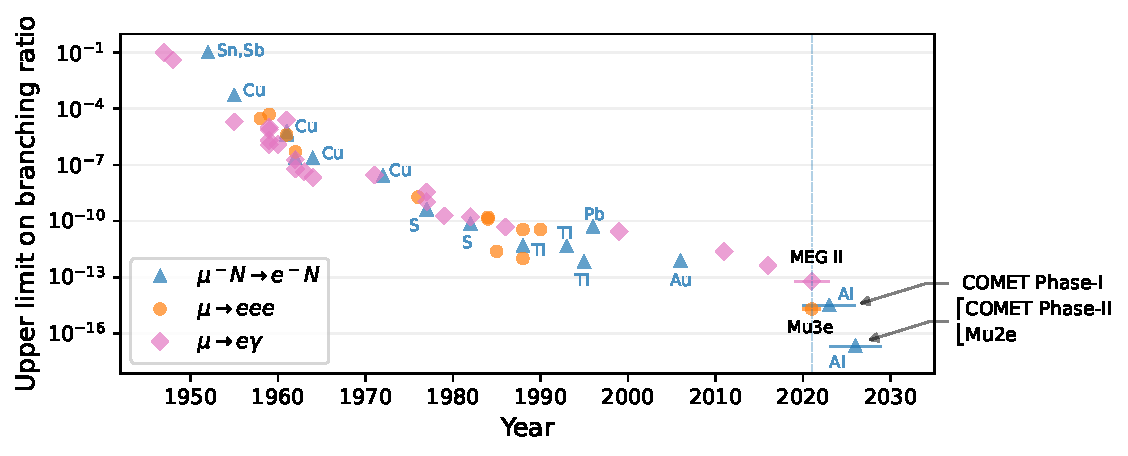
\includegraphics[width=\textwidth]{chapter1/clfv_upper_limit_v2.pdf}
    \caption{
        90\%-confidence upper limit on the branching ratio of three charged
        lepton flavour-violating processes over time. 
        The target material $N$ is indicated for $\mu$--$e$ conversion experiments.
        Past experiment results
        were tabulated in~\cite{BERNSTEIN201327}. Future data points are the
        expected sensitivities quoted in the MEG II~\cite{Baldini2018},
        Mu3e~\cite{ARNDT2021165679}, COMET
        Phase-I~\cite{the_comet_collaboration_comet_2020} and
        Mu2e~\cite{bartoszek2015mu2e} design reports.
    }
    \label{fig:clfv_upper_limit}
\end{figure}

\section{Muon to electron conversion}
% mu-e conversion
Muon to electron conversion is the neutrino-less decay of a muon bound to an
atomic nucleus:
$$
\mu^- + N(A, Z) \rightarrow e^- + N(A, Z),
$$
where $A$ is the mass number and $Z$ the atomic number.
Similarly to $\mu\rightarrow e+\gamma$, this process is allowed in the SM
extended with massive neutrinos via the diagram shown in
Fig.~\ref{fig:mu-e_conv_SM}, but suppressed to an experimentally
unreachable level. Any signs of it occurring at current experimental
sensitivities would suggest a BSM origin.

In order to search for this process, muons must be stopped in matter to form
muonic atoms. Initially bound in the outer atomic layers, the muon
electromagnetically cascades down to the $1s$ orbital within \SI{1}{\ns}
and gets in close range of the nucleus~\cite{Knecht2020}. 
When interacting with the nucleus, the reaction is called \emph{coherent} if the
nucleus remains in its ground state. For elements heavier than magnesium, the
ratio of coherent to incoherent $\mu$--$e$ conversion is expected to be around
9:1~\cite{CHIANG1993526}.

In a coherent $\mu$--$e$ conversion, the kinematics are those of a
straightforward two-body decay, hence the electron always has an energy
\begin{equation*}\label{eq:mu_e_conv_energy}
E_{\mu\text{--}e} = m_\mu - B_\mu - E_\mathrm{recoil},
\end{equation*}
where $B_\mu$ is the binding energy of the $1s$-state muonic atom and
$E_\mathrm{recoil}$ is the recoil energy of the nucleus. In aluminium, the
target material of the COMET and Mu2e experiments, this yields
$$
    E^\mathrm{Al}_{\mu\text{--}e} = \SI{104.97}{\MeV}.
$$
Since the signature of $\mu$--$e$ conversion is a single, mono-energetic
electron, this process should be relatively easily identified by means of a
momentum-measuring detector. However, this signal must also be discriminated
from backgrounds originating from other processes, contamination of the beam and
cosmic rays.

\subsection{Standard Model backgrounds}
\subsubsection{Decay in orbit}
In the SM, a bound muon is allowed to decay in orbit (DIO):
\begin{equation*}\label{eq:dio}
    \mu^- + N(A, Z) \rightarrow e^- + \nu_\mu + \overline{\nu}_e + N(A, Z).
\end{equation*}
Although the process is the same as a free decay, shown in
Fig.~\ref{fig:weak_decay}, here the nucleus is also involved in the kinematics
of the process. In a free decay, the electron may carry at most half of the muon
mass as kinetic energy (in the muon rest frame) when the two neutrinos are
emitted in the opposite direction. In DIO, the nucleus can recoil and
potentially provide more energy to the electron. If the two neutrinos are
emitted back to back in the transverse direction to the electron, then the
kinematics resemble that of $\mu$--$e$ conversion and the electron could easily
be mistaken for the CLFV signal. 

% Mention muon lifetime in orbit?

The energy spectrum of DIO electrons for various target nuclei is well
understood theoretically~\cite{czarnecki}, hence the expected background rate
for $\mu$--$e$ conversion searches is precisely known. Although it is extremely
unlikely that a DIO electron might carry as much energy as a conversion
electron, the sensitivity aimed at by future experiments makes DIO the main
background source and sensitivity-limiting
factor~\cite{the_comet_collaboration_comet_2020}.


\subsubsection{Nuclear capture}
A muon in proximity with a nucleus may also be captured via $W$-boson exchange:
\begin{equation*}\label{eq:capture}
    \mu^- + N(A, Z) \rightarrow \nu_\mu + N(A, Z-1).
\end{equation*}
This process is similar to an electron capture and transmutes the nucleus into a
potentially unstable isotope, which can be the source of proton, photon and
neutron emissions as it readjusts. Particles emitted by the nucleus after muon
capture may hit and damage the readout electronics if they are close to the
target, as is the case in COMET Phase-I. The AlCap experiment, performed in 2013
at the Paul Scherrer Institute, measured the spectrum of particles emitted after
capture of stopped muons by aluminium, titanium and silicon
nuclei~\cite{PhysRevC.105.035501}.


Radiative muon capture (RMC) occurs when a photon is emitted during the capture
process. Kinematically, the photon can carry energies close to the muon mass,
hence if it produces an electron--positron pair with asymmetric momenta, the
electron will mimic the conversion signal. The high-energy endpoint of the RMC
spectrum is not as high as for DIO, hence an adequate momentum resolution from a
tracking detector will discriminate most RMC electrons from the signal. In COMET
Phase-I, the background rate from RMC is 5 times lower than that from
DIO~\cite{the_comet_collaboration_comet_2020}.




Sources of background other than DIO and nuclear capture are expected in
$\mu$--$e$ conversion-searching experiments, such as beam-related and cosmic
ray-induced events. All backgrounds specific to the COMET experiment, and the
associated design choices which were made to minimise their occurrence, are
discussed in Section~\ref{sec:backgrounds}.






\section{Effective CLFV and the scale of new physics}
Experiments searching for CLFV are sensitive to a wide variety of new physics,
including a non-minimal Higgs, a $Z'$ boson, leptoquarks, heavy neutrinos, or
supersymmetric particles. 
In order to determine the scale of new physics to which future CLFV-searching
experiments will be sensitive and the complementarity between experiments, we can
consider a low-energy effective field theory derived from new interactions with
generic massive ($m>\SI{1}{\tera\eV}$) particles.
After integrating out heavy fields (see
e.g.~\cite[Chapter~IV]{donoghue_golowich_holstein_2014}), one obtains the
following effective Lagrangian~\cite{DEGOUVEA201375}, which allows CLFV to be
mediated by the tree-level vertices shown in Fig.~\ref{fig:tree_lvl_clfv}:
\begin{align}\label{eq:Leff}
    \mathcal{L^\text{eff}_\mathrm{CLFV}}\,
    =\,
    &\frac{1}{\kappa+1}\, \frac{m_\mu}{\Lambda^2}\,\,
    \overline{\mu}_R \sigma_{\mu\nu} e_L \, F^{\mu\nu} + \text{h.c.}
    \nonumber\\[1em]
    +\,
    &\frac{\kappa}{\kappa+1}\, \frac{1}{\Lambda^2}\,\,
    \overline{\mu}_L \gamma_\mu e_L \,
    (\,
        \overline{u}_L \gamma^\mu u_L + \overline{d}_L \gamma^\mu d_L
    \,) + \text{h.c.}
\end{align}
where both interactions are suppressed by factors of $\Lambda$, the energy scale
of the new physics, and $\kappa$ determines whether the preferred channel is
photonic ($\kappa \rightarrow 0$) or four-fermionic ($\kappa \rightarrow
\infty$)~\cite{DEGOUVEA201375}. The $\kappa$ parameter allows this Lagrangian to
be model independent, i.e.\ it gives freedom for the new interaction to either
enhance $\mu \rightarrow e\gamma$ or $\mu$--$e$ conversion more strongly.
Searches for $\mu \rightarrow e\gamma$ will be more sensitive to CLFV than
$\mu$--$e$ conversion searches if $\kappa \ll 1$, whereas the opposite is true
if $\kappa \gg 1$.

\begin{figure}
    \centering
    \begin{subfigure}[b]{0.3\textwidth}
        \centering
        \feynmandiagram [small, inline=(b.base), vertical=b to d] {
            a [particle=\(\mu^{-}\)] -- [fermion] b [blob]
            -- [fermion] c [particle=\(e^-\)],
            b -- [boson] d [particle=\(\gamma\)],
        };
        \caption{Photonic}
    \end{subfigure}
    \hspace{1cm}
    \begin{subfigure}[b]{0.3\textwidth}
        \centering
        \feynmandiagram [small, inline=(b.base), vertical=a to d] {
            a [particle=\(\mu^{-}\)] -- [fermion] b [blob]
            -- [fermion] {c [particle=\(e^-\)],
            e [particle=\(q\)]},
            d [particle=\(q\)] -- [fermion] b,
        };
        \caption{Four-fermionic}
    \end{subfigure}
    \caption{New vertices which arise in the effective Lagrangian of
    Eq.~\ref{eq:Leff} and allow CLFV. The photonic interaction can also mediate
    $\mu$--$e$ conversion by making the photon interact with an external quark.}
    \label{fig:tree_lvl_clfv}
\end{figure}

From the estimated sensitivity of a future experiment, we can estimate the
maximum scale of new physics $\Lambda$ which the experiment will be able to
probe. COMET Phase-II and Mu2e, which have a single-event sensitivity of around
$10^{-17}$~\cite{the_comet_collaboration_comet_2020, bartoszek2015mu2e}, will
probe energy scales $\Lambda$ up to \SI{4000}{\tera\eV} if $\kappa$ is small and up to
\SI{7000}{\tera\eV} if $\kappa$ is large~\cite{ben_thesis, ewen_thesis}. 

Even in the situation where no positive signal is observed, probing these enormous
energy scales will heavily constrain any model which predicts new heavy
particles whose interactions allow any significant amount of CLFV. On the other
hand, if CLFV is observed in either the $\mu\rightarrow e\gamma$ or $\mu$--$e$
conversion channels, the value of $\kappa$ can then be determined from a
measurement in the other channel. This data can then further constrain and
disambiguate models, and help to pinpoint the true nature of the new physics.

\section{Related experiments}
Charged lepton flavour violation is but one of the many properties of leptons
currently scrutinised by experiments. Related but orthogonal measurements
include the muon magnetic moment and lepton universality. From their results, it
is impossible to predict whether CLFV will appear, but they are complementary in
constraining the models of new physics which could lead to the observed
discrepancies.

The Muon $g-2$ experiment at Fermilab recently observed a $4.2\sigma$
discrepancy between the Standard Model prediction and the measured value for the
magnetic moment of the muon~\cite{PhysRevLett.126.141801}. This deviation,
assuming it is a true sign of new physics\footnote{
    The theoretical expectation for the SM magnetic moment is disputed by a
    different approach using lattice QCD~\cite{Borsanyi2021}. The latter calculation
    is indeed more consistent with the measurement, hence further investigation is
    necessary to understand the cause of the initial discrepancy and why the two
    calculations disagree.
}, could be attributed to various scenarios where new particles, e.g.\ 
leptoquarks, a new Higgs doublet or neutral boson, interact with the muon.


The LHCb experiment at CERN has found evidence for lepton non-universality in
the decay of b-quarks, with a significance of $3.1\sigma$~\cite{Aaij2022}. As
with the $g-2$ discrepancy, models which could explain the anomaly include a
heavy neutral boson, leptoquarks, or an extended Higgs sector. 

Together, the Muon $g-2$ and LHCb results suggest a tension related to a special
property of the muon, which would differentiate it from the electron in a new,
unexplained way. Although there are so far no tangible traces of CLFV, models
attempting to resolve the $g-2$ and LHCb anomalies often also allow CLFV at some
level~\cite{DEGOUVEA201375, PhysRevD.101.115016, PhysRevD.100.115010}. Hence,
measurements such as the $\mu$--$e$ conversion branching ratio are crucial to
further constrain models and guide the theory toward the true nature of the new
physics.
